% put all of your slides that you want to create in here 

\section{Problemstellung und Ansatz}

\begin{frame}
    \frametitle{Problem}

    \begin{itemize}
        \item \acp{TEA} sind durch Covert-Channel begrenzt\\
        \textrightarrow\space \ac{CPU}-Rollback erfordert zwangsläufig Übertragung
        \item \ac{CbCC} häufig verwendet \cite[23]{xiong_survey_2022} \textrightarrow\space hoher Durchsatz mit geringer Komplexität
        \item Abhängigkeit der Laufzeit von Übertragungen von Datenmenge und Durchsatz\\
        \textrightarrow\space Durchsatz vorrangig durch Covert-Channel bestimmt
    \end{itemize}
    \note{- TEAs durch Übertragung begrenzt (da Rollback praktisch einen Angriff definiert)}
    \note{- CbCC meist verwendet -> Durchsatz, Komplexität, meist hardwareunabhängig, viel Literatur...}
    \note{- Laufzeit ergibt sich aus Größe übertragener Daten und Durchsatz}
    \note{- Menge Daten abhängig von konkretem Angriff -> Durchsatz abhängig von Covert Channel -> allgemeingültig (besonders Encodierung, Rest begrenzt durch technische Grenzen)}
    \note{Fragestellung: Grenze von CbCC bei TEAs was die Laufzeit (damit Durchsatz) angeht}

    \pause
    \vspace{0.5cm}

    \begin{block}{Fragestellung}
        Wo liegt die Grenze für \ac{CbCC} im Kontext von \acp{TEA}
        hinsichtlich der Laufzeit und damit hinsichtlich des Durchsatzes?
    \end{block}

\end{frame}

\begin{frame}
    \frametitle{Ansatz}

    \begin{itemize}
        \item häufig Array-Index Encodierung für \acp{CbCC}
        \item bitweise Encodierung bisher nicht implementiert oder getestet\\
        \textrightarrow\space nur Kombination aus beiden \cite{hertogh_rain_nodate}
    \end{itemize}

    \note{- bisherige Angriffe nutzen meist Array-Index Enc. -> Ausnahme l1tf reloaded -> Encodierung 1 Byte als 2x 16 Adressen -> keine reine bitweise Enc. -> Grenzen nicht getestet}
    \note{- reine bitweise Encodierung nicht betrachtet}

    \pause

    \begin{columns}[t]
        \begin{column}{0.4\textwidth}
            \begin{block}{Ziel 1}
                Implementieren von Bitweiser Encodierung während Transient Execution,
                um die Umsetzbarkeit verschiedener Encodierungen zu zeigen.
                Zusätzlich können Aspekte wie Genauigkeit und Laufzeit betrachtet werden.
            \end{block}
        \end{column}
        \note{- Implementierung beider Implementierungen, um grundsätzliche Umsetzbarkeit zu testen}
        \note{- Erster Vergleich bitweise und Array-Index Encodierung}
        \pause
        \begin{column}{0.4\textwidth}
            \begin{block}{Ziel 2}
                Modellierung der Laufzeit einer Übertragung sowie des Durchsatzes.
                Ermittlung einer Grenze für \acp{CbCC} während Transient Execution.
            \end{block}
        \end{column}
        \note{- Laufzeitbetrachtung mit Entwicklung einer Funktion}
        \note{- ermitteln einer Grenze der Laufzeit / vom Durchsatz von CbCC}
    \end{columns}

\end{frame}

\begin{frame}
    \frametitle{Phasen des Angriffs}

    \begin{itemize}
        \item wegen grundsätzlicher Funktionsweise bestehen \acp{TEA} aus 3 Phasen
        \item bei konkretem Angriff wiederholen dieser Phasen \textrightarrow\space stückweises übertragen von Secret
        \item Optimieren dieser Phasen für kürzere Laufzeiten
    \end{itemize}

    \pause
    \vspace{0.5cm}

    \begin{figure}
        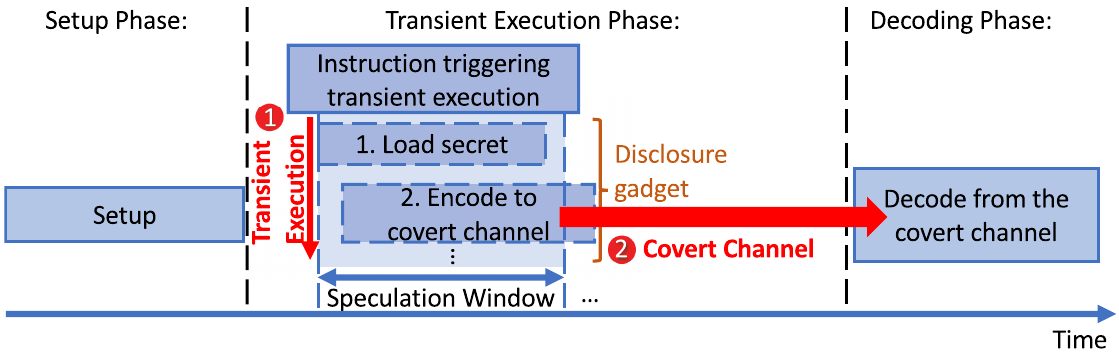
\includegraphics[width=\textwidth]{img/transient-attack-phases.png}
        \caption{Phases of transient execution attacks. \cite[2]{xiong_survey_2022}}
    \end{figure}

    \note{Erklärung Unterschied von Side und Covert Channel (Encode bewusst, unbewusst)}

\end{frame}

\section{Umsetzung und Ergebnisse}

\begin{frame}
    \frametitle{CbCC Laufzeit}

    \only<1>{
        \note{- Unterscheidung bitweise und Array-Index Encodierung -> Ursprünglich erstmals unterschieden in zitierter Quelle}
        \note{- Andere Benennung für Encodierung: Bitweise -> Direct-mapped bits; Array-Index -> Index values}
        \note{- Encodierung von 0 bei Index values als seperater Zustand}
        \note{- binäre Darstellung least signigicant bit first (von links nach rechts)!!!!}
        \note{- Erklären wie die Adressen im folgenden dargestellt (gelbe \& grüne Kästchen)}
    }
    \tikzset{shape address/.style = {
        shape=rectangle, color=black, draw,
        outer xsep=0.1cm, outer ysep=0.1cm,
        fill=yellow!40,
    }}
    \begin{block}{Beispiel: Encodierung des Werts $7$ ($1110_2$) in vier Bit (Encodierungen ähnlich zu \cite{mcilroy_spectre_2019})}
        \pause
        \begin{columns}
            \begin{column}{0.49\textwidth}
                \textbf{Bitweise:}\\
                \begin{tikzpicture}
                    \node[shape address, fill=green!60] (adr1) {};
                    \node[shape address, fill=green!60] (adr2) [right=0cm of adr1.east] {};
                    \node[shape address, fill=green!60] (adr3) [right=0cm of adr2.east] {};
                    \node[shape address] (adr4) [right=0cm of adr3.east] {};
                \end{tikzpicture}
            \end{column}
            \pause
            \begin{column}{0.49\textwidth}
                \textbf{Array-Index:}\\
                \begin{tikzpicture}
                    \node[shape address] (adr1) {};
                    \node[shape address] (adr2) [right=0cm of adr1.east] {};
                    \node[shape address] (adr3) [right=0cm of adr2.east] {};
                    \node[shape address] (adr4) [right=0cm of adr3.east] {};
                    \node[shape address] (adr5) [right=0cm of adr4.east] {};
                    \node[shape address] (adr6) [right=0cm of adr5.east] {};
                    \node[shape address, fill=green!60] (adr7) [right=0cm of adr6.east] {};
                    \node[shape address] (adr8) [right=0cm of adr7.east] {};
                    \node[shape address] (adr9) [right=0cm of adr8.east] {};
                    \node[shape address] (adr10) [right=0cm of adr9.east] {};
                    \node[shape address] (adr11) [right=0cm of adr10.east] {};
                    \node[shape address] (adr12) [right=0cm of adr11.east] {};
                    \node[shape address] (adr13) [right=0cm of adr12.east] {};
                    \node[shape address] (adr14) [right=0cm of adr13.east] {};
                    \node[shape address] (adr15) [right=0cm of adr14.east] {};
                \end{tikzpicture}
            \end{column}
        \end{columns}

        \only<2>{
            \note{- bitweise Encodierung sehr Intuitiv}
            \note{- praktisch encodieren durch Bitmask und load nach Branch}
        }
        \only<3>{
            \note{- Array Index Intuitiv}
            \note{- Auch Bitmask (nur betrachtete Bits übertragen)}
            \note{- Wert als Offset bei einer Load Instruktion}
            \note{}\note{---}
            \note{- bitweise nur so viele Adressen nötig, wie encodiert}
            \note{- Array-Index exponentielle Anzahl an Adressen -> flushen und messen}
        }
        \pause
        \vspace{1cm}

        \textbf{Kombination mit Parametern $n_b=2$ und $n_a=2$:}\\
        \begin{tikzpicture}

            \node[shape address, fill=green!60] (adrb1) [] {};
            \node[shape address, fill=green!60] (adrb2) [right=0cm of adrb1.east] {};
            \node[shape address, fill=green!60] (adrb3) [right=0cm of adrb2.east] {};
            \node[shape address] (adrb4) [right=0cm of adrb3.east] {};
            \onslide<5->{
                \node[shape address] (adr11) [below=0.5cm of adrb1.south] {};
                \node[shape address] (adr12) [right=0cm of adr11.east] {};
                \node[shape address, fill=green!60] (adr13) [right=0cm of adr12.east] {};
                \node[] (split1) [right=0cm of adr13.east] {|};
                \node[shape address, fill=green!60] (adr21) [right=0cm of split1.east] {};
                \node[shape address] (adr22) [right=0cm of adr21.east] {};
                \node[shape address] (adr23) [right=0cm of adr22.east] {};
                \begin{scope}[local bounding box=bracket1]
                    \draw[decorate, decoration = {calligraphic brace}] (adrb2.south) -- (adrb1.south);
                \end{scope}
                \begin{scope}[local bounding box=bracket2]
                    \draw[decorate, decoration = {calligraphic brace}] (adrb4.south) -- (adrb3.south);
                \end{scope}
                \draw[->] (bracket1.south) -- (adr13.north);
                \draw[->] (bracket2.south) -- (adr21.north);
            }
        \end{tikzpicture}
        \only<4-5>{
            \note{- Encodierung von n\_a Bits in n\_b Gruppen}
            \note{}\note{---}
            \note{- in diesem Falle immer 2 Bit als Array Index Encodierung}
            \note{- hohe Komplexität (Bitmaske mit n\_a Bit -> schiften und jedes Mal Index encodieren)}
        }
        \onslide<6->{
            \note{- Herleitung Formeln erklären (für reine bitweise und Array-Index Encodierung)}
            \note{- Anzahl an Adressen n\_a wird n\_b mal ausgeführt}
        }
    \end{block}

    \pause
    \pause

    \only<6>{
        \begin{center}
            $N_P=n_b*(2^{n_a}-1)$\hspace{1cm}$N_R=n_b*2^{n_a-1}$
        \end{center}

        \begin{itemize}
            \item Array-Index encodiert $0$ als keine gecachte Adresse \textrightarrow\space vereinfacht die Formel
            \item vorbereitete Adressen und gemessene Adressen wird unterschieden \textrightarrow\space
            dafür keine Betrachtung des Zeitunterschieds von gecachten und ungecachten Adressen
            \item obere Grenze für Durchsatz, da bei entsprechend verwendeten Parametern die Laufzeit unterschätzt wird
        \end{itemize}
    }

\end{frame}

\begin{frame}
    \frametitle{Genauigkeit und Parameter}

    \only<1>{
        \begin{columns}
            \begin{column}{0.5\textwidth}
                \begin{figure}[H]
                    \begin{tikzpicture}
                        \begin{axis}[
                                width=\textwidth,
                                scaled ticks=false,
                                xlabel={$n_b$},
                                ylabel={Genauigkeit},
                                xmin=0,xmax=32,
                                ymin=0,ymax=1,
                            ]
                            \addplot+ [
                                id=runtime,
                                smooth,
                                domain=0:10,
                            ] coordinates{
                                (1, 0.99) (2, 0.96) (3, 0.97) (4, 0.93) (5, 0.91) (6, 0.87) (7, 0.91) (8, 0.92) (9, 0.87) (10, 0.9) (11, 0.92) (12, 0.86) (13, 0.66) (14, 0.35) (15, 0.16) (16, 0.08) (17, 0.05) (18, 0.03) (19, 0.03) (20, 0.01) (21, 0.01) (22, 0.01) (23, 0.0) (24, 0.0) (25, 0.0) (26, 0.0) (27, 0.0) (28, 0.0) (29, 0.0) (30, 0.0) (31, 0.0) (32, 0.0)
                            };
                        \end{axis}
                    \end{tikzpicture}
                    \caption{grafische Ermittlung von $n_{bmax}$ durch absolute Genauigkeit}
                \end{figure}
            \end{column}
            \begin{column}{0.5\textwidth}
                \begin{itemize}
                    \item bestimmen von $n_{bmax}$ grafisch
                    \item Messen Genauigkeit abhängig von $n_b$ ($n_a=1$)
                    \item abschätzen Maximalwert $n_{bmax}$
                \end{itemize}
            \end{column}
        \end{columns}
    }

\end{frame}

\begin{frame}
    \frametitle{Laufzeit der kombinierten Encodierung}

    \note{- etwa Faktor 20 geringer als berechnet}
    \note{- keine Betrachtung der Genauigkeit}
    \note{- genauere Einschätzung des Durchsatzes möglich}

    \begin{figure}[H]
        \begin{tikzpicture}
            \begin{axis}[
                    height=0.8\textheight,
                    xtick distance=1,
                    scaled ticks=false,
                    xlabel={$n_a$},
                    xmin=0,xmax=10,
                    ymin=0,ymax=0.0013,
                    axis y line*=left,
                    ylabel style = {at={(axis description cs:-0.25,.5)}},
                    ylabel={Berechnung \ref{pgfplots:plot1}},
                    xmajorgrids,
                ]
                \addplot+ [
                    id=runtime,
                    smooth,
                    domain=0:10,
                ] plot (\x, {(10*\x)/((20*109) + 569 + (10*144*2^(\x)-1) + (10*410*2^(\x-1)))});
                \label{pgfplots:plot1}
            \end{axis}
            \onslide<2->{
                \begin{axis}[
                        height=0.8\textheight,
                        xtick distance=1,
                        scaled ticks=false,
                        xlabel={$n_a$},
                        xmin=0,xmax=10,
                        ymin=0,ymax=0.00006,
                        axis y line*=right,
                        ylabel style = {align=center},
                        ylabel={Messung \ref{pgfplots:plot2}}
                    ]
                    \addplot+ [
                        id=runtime,
                        smooth,
                        red,
                        mark options={
                            fill=red,
                        },
                        domain=0:10,
                    ] coordinates {
                        (1, 4.3057799584543905e-05) (2, 5.2178130397583005e-05) (3, 4.8291788256670144e-05) (4, 3.5208914559160803e-05) (5, 2.401284283676007e-05) (6, 1.716950947051971e-05)
                    };
                    \label{pgfplots:plot2}
                \end{axis}
            }
            \onslide<3->{
                \begin{axis}[
                        height=0.8\textheight,
                        xtick distance=1,
                        scaled ticks=false,
                        xlabel={$n_a$},
                        xmin=0,xmax=10,
                        ymin=0,ymax=0.0013,
                        axis y line*=left,
                        ylabel style = {at={(axis description cs:-0.35,.5)}},
                        ylabel={Messung 2 \ref{pgfplots:plot3}}
                    ]
                    \addplot+ [
                        id=runtime,
                        smooth,
                        green,
                        mark options={
                            fill=green,
                        },
                        domain=0:10,
                    ] coordinates {
                        (1, 5.621827216401164e-05) (2, 9.440744013706828e-05) (3, 0.00012123838218047957) (4, 0.0001341703865965394) (5, 0.0001219833219522894) (6, 0.00010153788777128956)
                    };
                    \label{pgfplots:plot3}
                \end{axis}
            }
        \end{tikzpicture}
        \caption{$D(n_a)$ mit $N_T=20$, $T_T=109$, $L_E=569$,
            $T_P=144$, $T_R=410$ und $n_{bmax}=10$}
    \end{figure}

\end{frame}

\section{Ausblick}

\begin{frame}
    \frametitle{Genauigkeit \& Fehlerkorrekturen}

    \begin{itemize}
        \item nur Betrachtung von reiner Laufzeit \textrightarrow\space Annahme keine Fehler
        \item praktisch betrachtet Fehlerkorrektur nötig \textrightarrow\space stark abhängig von Encodierung
    \end{itemize}

    \only<1>{
        \note{- in dieser Arbeit nur Betrachtung der Laufzeit}
        \note{- für realistischen Durchsatz müsste Fehlerwahrscheinlichkeit und Fehlerkorrektur betrachtet werden}
        \note{- Betrachtung Fehlerkorrektur abhängig von Hardware -> wahrscheinlich komplex (Anzahl ausführbarer Instruktionen)}
        \note{- einfachste "naive" Fehlerkorrektur durch wiederholtes Ausführen -> Häufigkeit analysieren}
    }
    \pause

    \begin{columns}[t]
        \begin{column}{0.45\textwidth}
            \begin{block}{Bitweise Encodierung}
                \begin{itemize}
                    \item theoretisch unabhängige Datenpunkten\\
                    \textrightarrow\space jeweils Fehlerkorrektur
                    \item da unabhängige Daten sind komplexere Verfahren möglich\\
                    \textrightarrow\space fraglich, ob praktisch effizient (während Transient Execution)
                \end{itemize}
            \end{block}
        \end{column}
        \pause
        \begin{column}{0.45\textwidth}
            \begin{block}{Array-Index Encodierung}
                \begin{itemize}
                    \item Betrachtung der häufigsten Werte möglich\\
                    \textrightarrow\space $0$ als Index encodieren\\
                    \textrightarrow\space alle Adressen messen
                    \item weniger übertragene unabhängige Informationen\\
                    \textrightarrow\space weniger Möglichkeiten als bitweise
                \end{itemize}
            \end{block}
        \end{column}
    \end{columns}

    \only<2>{
        \note{- Vorteil theoretisch unabhängiger Datenpunkte}
        \note{- jeweils naive Fehlerkorrektur möglich}
        \note{- komplexer wie durch Parität oder 2x mal übertragen möglich}
        \note{- mehr Instruktionen für Fehlerkorrektur durch Transient Window begrenzt -> nur sehr eingeschränkt möglich -> Nutzen fraglich}
    }
    \only<3>{
        \note{- naive Fehlerkorrektur -> sowohl lesen bis Adresse gecached oder alle lesen möglich}
        \note{-> im Idealfall alle Adressen messen -> höhere Laufzeitkomplexität (2\^n anstatt 2\^(n-1))}
        \note{- 0 sollte als seperater Zustand encodiert werden (könnte statistisch wahrscheinlich auch modelliert werden, wenn alle Adressen messen) -> Änderung der Formeln nötig}
        \note{- generell weniger unabhängige Informationen -> Fehlerkorrektur noch eingeschränkter (nicht nur Transient Window, auch Encodierung)}
    }

\end{frame}
